% Why New York? Density and possibility
% Compile with: latexmk -pdf general_nyc.tex
\documentclass[aspectratio=169,11pt]{beamer}

\usepackage[T1]{fontenc}
\usepackage{lmodern}
\usepackage{booktabs}
\usepackage{array}
\usepackage{tikz}
\usetikzlibrary{shapes.geometric,positioning,calc,arrows.meta}
\usepackage{pgfplots}
\pgfplotsset{compat=1.18}
\usepackage[most]{tcolorbox}
\graphicspath{{images/}}

% ---------- Colors ----------
\definecolor{navy}{HTML}{1C2541}
\definecolor{oldred}{HTML}{B22234}   % US flag red, also the accent color
\definecolor{oldblue}{HTML}{3C3B6E}  % US flag blue
\definecolor{ink}{HTML}{2B2B2B}
\definecolor{muted}{HTML}{8A8F98}
\definecolor{paper}{HTML}{FFFFFF}
\definecolor{dem}{HTML}{2E5FA3}      % Democrats
\definecolor{rep}{HTML}{C0392B}      % Republicans
\definecolor{austria}{HTML}{C8102E}  % Austria red, for USA-vs-Austria comparisons

% ---------- Minimal theme ----------
\setbeamertemplate{navigation symbols}{}
\setbeamercolor{normal text}{fg=ink, bg=paper}
\setbeamercolor{structure}{fg=navy}
\setbeamercolor{frametitle}{fg=navy}
\setbeamercolor{alerted text}{fg=oldred}
\setbeamercolor{footnote}{fg=muted}
\setbeamerfont{frametitle}{size=\Large, series=\bfseries}
\setbeamertemplate{itemize item}{\color{oldred}\textbullet}
\setbeamertemplate{itemize subitem}{\color{muted}--}
\setbeamertemplate{enumerate item}{\color{oldred}\insertenumlabel.}
\setbeamersize{text margin left=1.1cm, text margin right=1.1cm}
\hypersetup{colorlinks=true, urlcolor=dem, linkcolor=navy}

\setbeamertemplate{frametitle}{%
  \vspace*{0.5cm}%
  \usebeamerfont{frametitle}\usebeamercolor[fg]{frametitle}\insertframetitle\par
  \vspace{0.15cm}{\color{navy!15}\rule{\textwidth}{0.4pt}}\par}

\setbeamertemplate{footline}{%
  \hfill{\tiny\color{muted}\insertframenumber}\hspace*{0.6cm}\vspace*{0.35cm}}

% Plain divider at the start of each section
\AtBeginSection{%
  \begin{frame}[plain,noframenumbering]
    \centering
    {\LARGE\bfseries\color{navy}\insertsection}\\[0.6em]
    {\color{oldred}\rule{1.5cm}{0.8pt}}
  \end{frame}}

% "Think" question slides: \begin{thinkframe} ... \end{thinkframe}
\newenvironment{thinkframe}{%
  \begin{frame}[plain,noframenumbering,environment=thinkframe]\centering\Large}{\end{frame}}

% ---------- Helpers ----------
% Small grey source line at the bottom of a frame
\newcommand{\source}[1]{%
  \begin{tikzpicture}[remember picture,overlay]
    \node[anchor=south west, font=\tiny, text=muted, text width=0.85\paperwidth, align=left]
      at ($(current page.south west)+(0.6cm,0.25cm)$) {#1};
  \end{tikzpicture}}

% Quote box with a thin red rule on the left; optional arg e.g. [fontupper=\itshape\small]
\newtcolorbox{textquote}[1][]{%
  enhanced, frame hidden, boxrule=0pt, sharp corners,
  colback=navy!4, borderline west={2pt}{0pt}{oldred},
  left=10pt, right=8pt, top=6pt, bottom=6pt, fontupper=\itshape, #1}

% Photo + name + short bio (use inside a column): \candidate{file}{Name}{bio}
\newcommand{\candidate}[3]{%
  \begin{minipage}[t]{\linewidth}\centering
    \includegraphics[height=3.5cm]{#1}\\[0.5em]
    {\large\bfseries\color{navy}#2}\\[0.4em]
    \begin{minipage}{0.9\linewidth}\raggedright\small #3\end{minipage}
  \end{minipage}}

% Big number with a caption (use inside a column): \bignum{color}{91\%}{caption}
\newcommand{\bignum}[3]{%
  \begin{minipage}[t]{\linewidth}\centering
    {\fontsize{34}{38}\selectfont\bfseries\color{#1}#2}\\[0.3em]
    {\small #3}
  \end{minipage}}

% US flag drawn in TikZ (hoist height = #1), e.g. \usflag{3cm}
\newcommand{\usflag}[1]{%
  \begin{tikzpicture}[x=#1, y=#1]
    \def\fly{1.9}
    \foreach \i in {0,...,12} {
      \pgfmathsetmacro{\c}{mod(\i,2)==0 ? 1 : 0}
      \ifdim\c pt=1pt
        \fill[oldred] (0,{1-(\i+1)/13}) rectangle (\fly,{1-\i/13});
      \else
        \fill[white] (0,{1-(\i+1)/13}) rectangle (\fly,{1-\i/13});
      \fi
    }
    \def\cw{0.76} \def\ch{0.5385}
    \fill[oldblue] (0,{1-\ch}) rectangle (\cw,1);
    \foreach \r in {1,...,9} {
      \pgfmathsetmacro{\isodd}{mod(\r,2)}
      \ifdim\isodd pt=1pt
        \foreach \k in {0,...,5}
          \node[star, star points=5, star point ratio=2.618, fill=white, inner sep=0pt,
                minimum size=0.0616*#1] at ({(2*\k+1)*\cw/12},{1-\r*\ch/10}) {};
      \else
        \foreach \k in {0,...,4}
          \node[star, star points=5, star point ratio=2.618, fill=white, inner sep=0pt,
                minimum size=0.0616*#1] at ({(2*\k+2)*\cw/12},{1-\r*\ch/10}) {};
      \fi
    }
    \draw[ink!30, line width=0.3pt] (0,0) rectangle (\fly,1);
  \end{tikzpicture}}

% Agree/disagree spectrum for "spectrum game" activities
\newcommand{\spectrum}{%
  
\begin{tikzpicture}
    \shade[left color=oldblue, right color=oldred, rounded corners=2pt] (0,0) rectangle (11,0.18);
    \node[anchor=north, font=\small, text=oldblue] at (0,-0.15) {Strongly disagree};
    \node[anchor=north, font=\small, text=muted] at (5.5,-0.15) {Neutral};
    \node[anchor=north, font=\small, text=oldred] at (11,-0.15) {Strongly agree};
    \fill[paper, draw=muted] (5.5,0.09) circle (2.5pt);
  \end{tikzpicture}}

% One statement per slide: \statement{number}{total}{text}
\newcommand{\statement}[3]{%
  \begin{frame}[plain]
    \vfill
    \begin{center}
      {\small\color{muted}Statement #1 of #2}\\[1.2em]
      {\LARGE\bfseries #3}
    \end{center}
    \vfill
    \begin{center}\spectrum\end{center}
    \vspace{1.2cm}
  \end{frame}}


% ---------- Deck helpers ----------
\newcommand{\credit}[1]{\\[0.2em]{\tiny\color{muted}#1\par}}
% Photo on the right, bullets on the left: \photoslide{Title}{image}{credit}{bullets}{source}
\newcommand{\photoslide}[5]{%
  \begin{frame}{#1}
    \begin{columns}[c]
      \begin{column}{0.48\textwidth}
        \begin{itemize}\setlength{\itemsep}{0.9em}
          #4
        \end{itemize}
      \end{column}
      \begin{column}{0.48\textwidth}
        \centering
        \includegraphics[width=\linewidth,height=5.6cm,keepaspectratio]{#2}
        \credit{#3}
      \end{column}
    \end{columns}
    \source{#5}
  \end{frame}}

% Thumbnail with label for the borough vote
\newcommand{\bthumb}[2]{\begin{minipage}[t]{0.19\textwidth}\centering
    \includegraphics[width=\linewidth]{thumb_#1}\\[0.3em]{\small\bfseries\color{navy}#2}\end{minipage}}
% Neighborhood marker on the Manhattan map: pixel x, pixel y (1280x1612 map), label x, label y, anchor, name
\newcommand{\hood}[6]{%
  \fill[oldred] (#1/1280,1-#2/1612) circle (1.8pt);
  \draw[oldred, thin] (#1/1280,1-#2/1612) -- (#3,#4);
  \node[anchor=#5, font=\footnotesize\bfseries, text=navy, inner sep=2pt] at (#3,#4) {#6};}

\begin{document}

% ---------- Title slide ----------
\begin{frame}[plain,t]
  \vspace{0.9cm}
  \hspace*{0.4cm}\begin{minipage}{0.8\textwidth}
    {\fontsize{30}{34}\selectfont\bfseries\color{navy} New York}\\[0.8em]
    {\Large\color{muted} Density and possibility}\\[0.6em]
    {\color{oldred}\rule{3cm}{1.5pt}}
  \end{minipage}
  \begin{tikzpicture}[remember picture,overlay]
    \node[anchor=south, inner sep=0pt] at (current page.south) {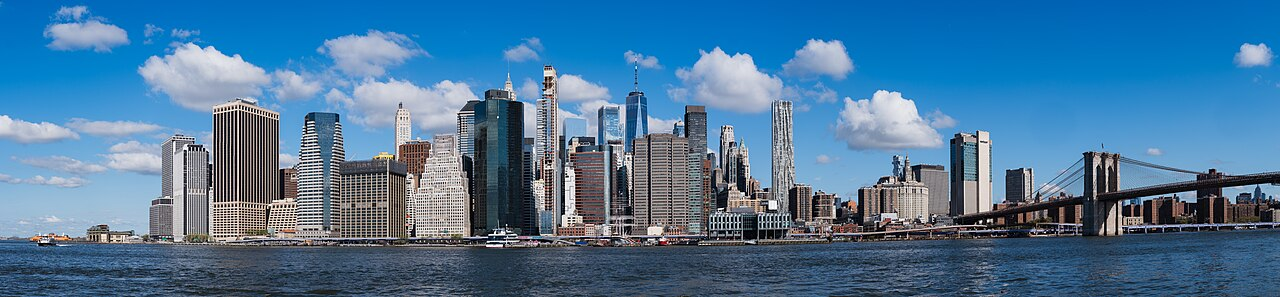
\includegraphics[width=\paperwidth]{skyline.jpg}};
    \node[anchor=south east, font=\tiny, text=white, inner sep=3pt] at (current page.south east) {Photo: Christian David, CC BY-SA 4.0};
  \end{tikzpicture}
\end{frame}

% =====================================================================
\section{Two Homes}

\begin{frame}{Guess the price}
  \begin{columns}[T]
    \begin{column}{0.47\textwidth}
      \centering
      {\large\bfseries\color{navy} Home A}\\[0.4em]
      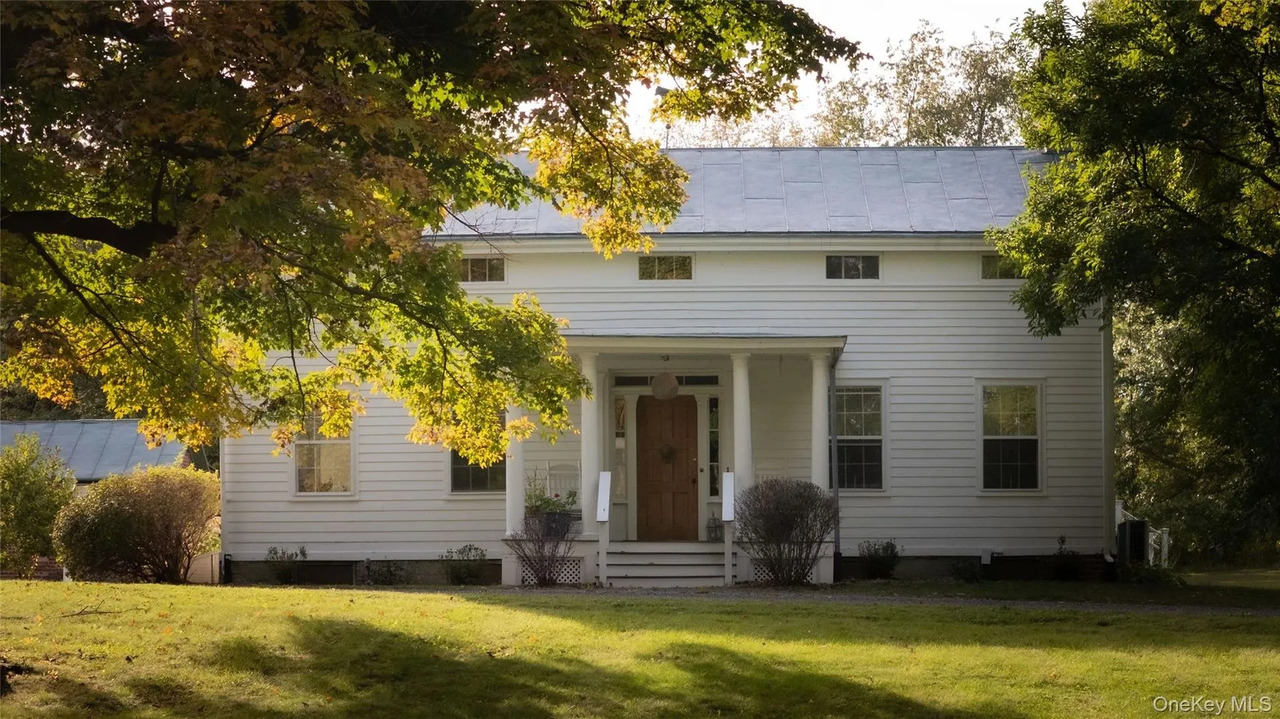
\includegraphics[height=3.8cm]{farmhouse_front.jpg}
    \end{column}
    \begin{column}{0.47\textwidth}
      \centering
      {\large\bfseries\color{navy} Home B}\\[0.4em]
      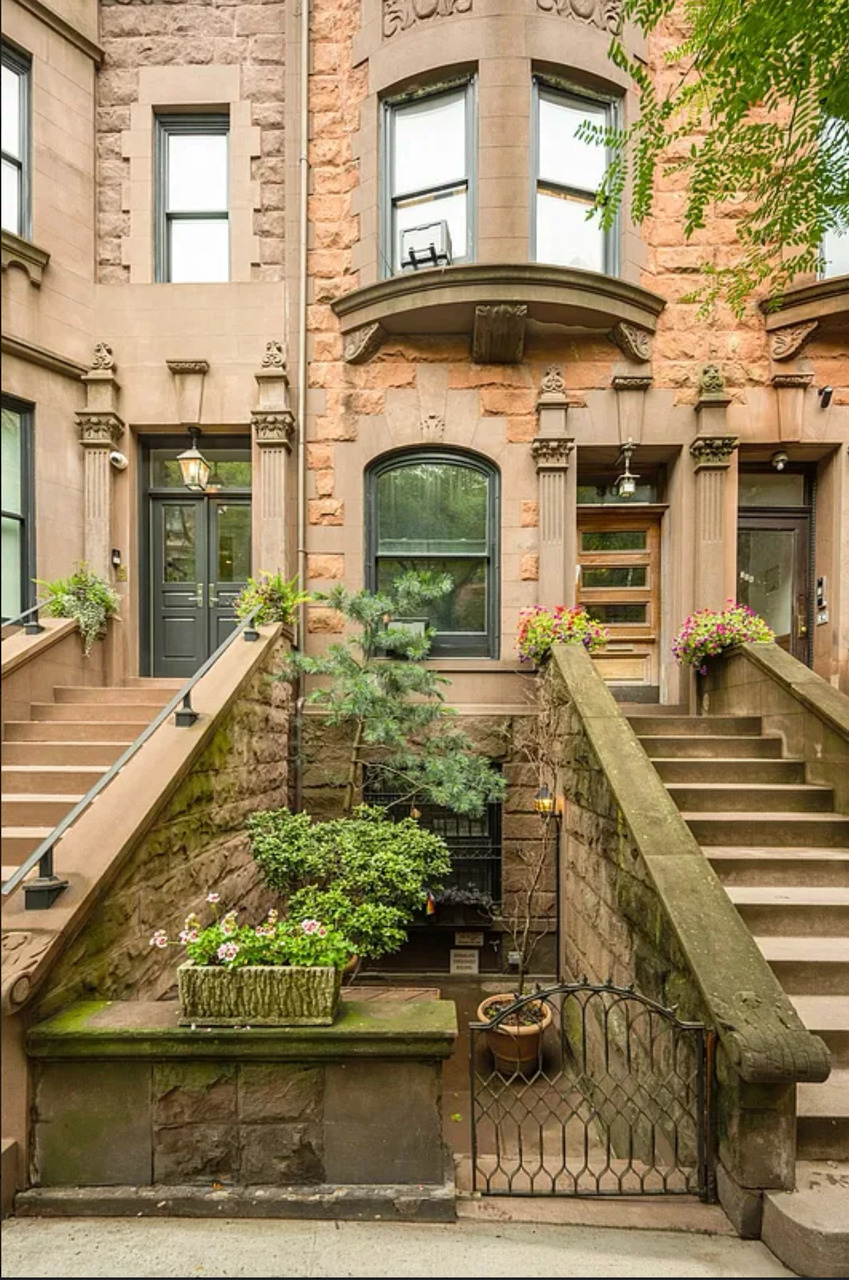
\includegraphics[height=3.8cm]{uws_listing.jpg}
    \end{column}
  \end{columns}
  \vspace{0.8em}
  \centering{\Large Which one costs \alert{more}?}
\end{frame}

\begin{frame}{Home A: the farmhouse}
  \begin{columns}[c]
    \begin{column}{0.44\textwidth}
      \begin{itemize}\setlength{\itemsep}{0.6em}
        \item Hudson, New York
        \item 4 bedrooms, 269 m\textsuperscript{2}
        \item Heated pool, 3-car garage
        \item 0.9 hectares of land
        \item Built around 1810
      \end{itemize}
      \vspace{0.6em}
      \uncover<2>{{\fontsize{26}{30}\selectfont\bfseries\color{oldred}\$1,200,000}}
    \end{column}
    \begin{column}{0.52\textwidth}
      \centering
      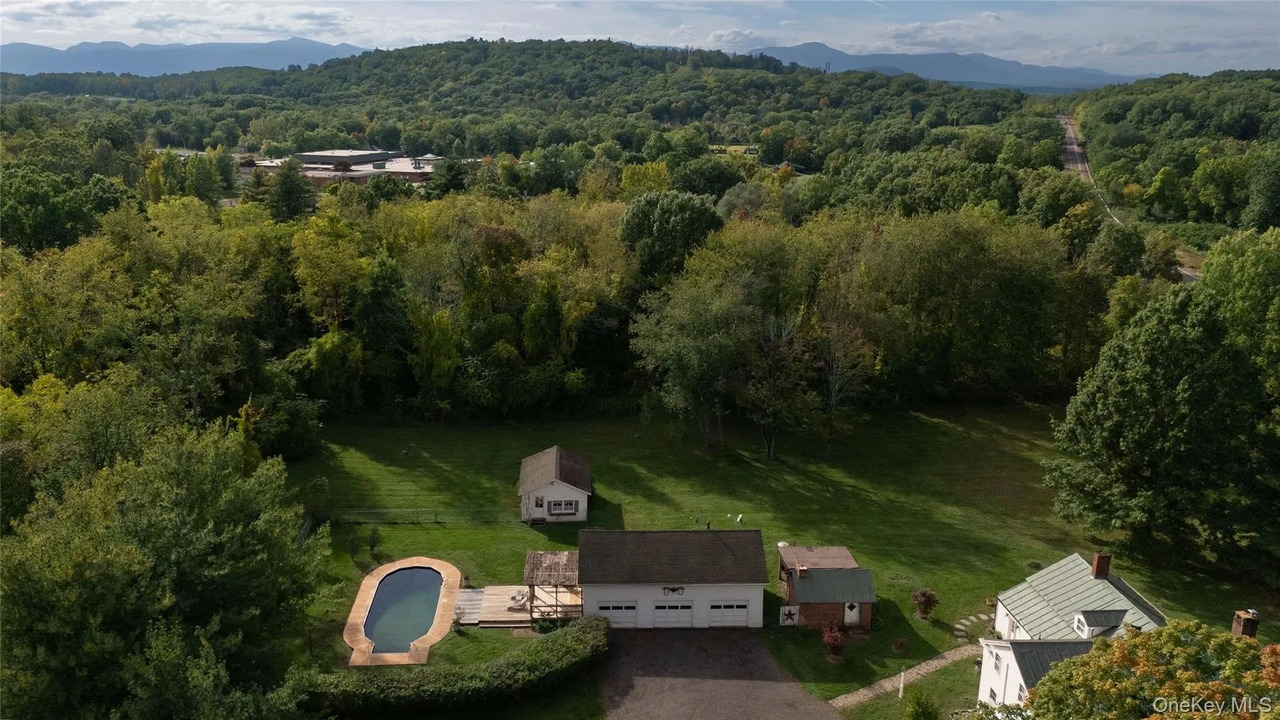
\includegraphics[width=\linewidth]{farmhouse_aerial.jpg}
      \credit{Listing photo: OneKey MLS}
    \end{column}
  \end{columns}
  \source{Source: \href{https://www.nestseekers.com/5535527/beautifully-renovated-farmhouse-on-22-private-acres-with-a-heated}{listing for 210 Middle Road, Hudson, NY} (Corcoran Country Living, Nov.\ 2026).}
\end{frame}

\photoslide{Hudson, New York}{hudson_warren.jpg}{Warren Street, Hudson. Photo: Acroterion, CC BY-SA 4.0}
  {\item Population: about \alert{6,000}
   \item Antique shops, farm-to-table restaurants
   \item Need a \alert{car} for everything
   \item New York City: 2 hours by train}
  {Source: US Census Bureau (2020: 5,894); Amtrak.}

\begin{frame}{Home B: the Manhattan apartment}
  \begin{columns}[c]
    \begin{column}{0.44\textwidth}
      \begin{itemize}\setlength{\itemsep}{0.6em}
        \item Upper West Side, Manhattan
        \item 2 bedrooms, 86 m\textsuperscript{2}
        \item A small private garden
        \item Plus \$2,217 a month in building fees
      \end{itemize}
      \vspace{0.6em}
      \uncover<2>{{\fontsize{26}{30}\selectfont\bfseries\color{oldred}\$1,250,000}}
    \end{column}
    \begin{column}{0.52\textwidth}
      \centering
      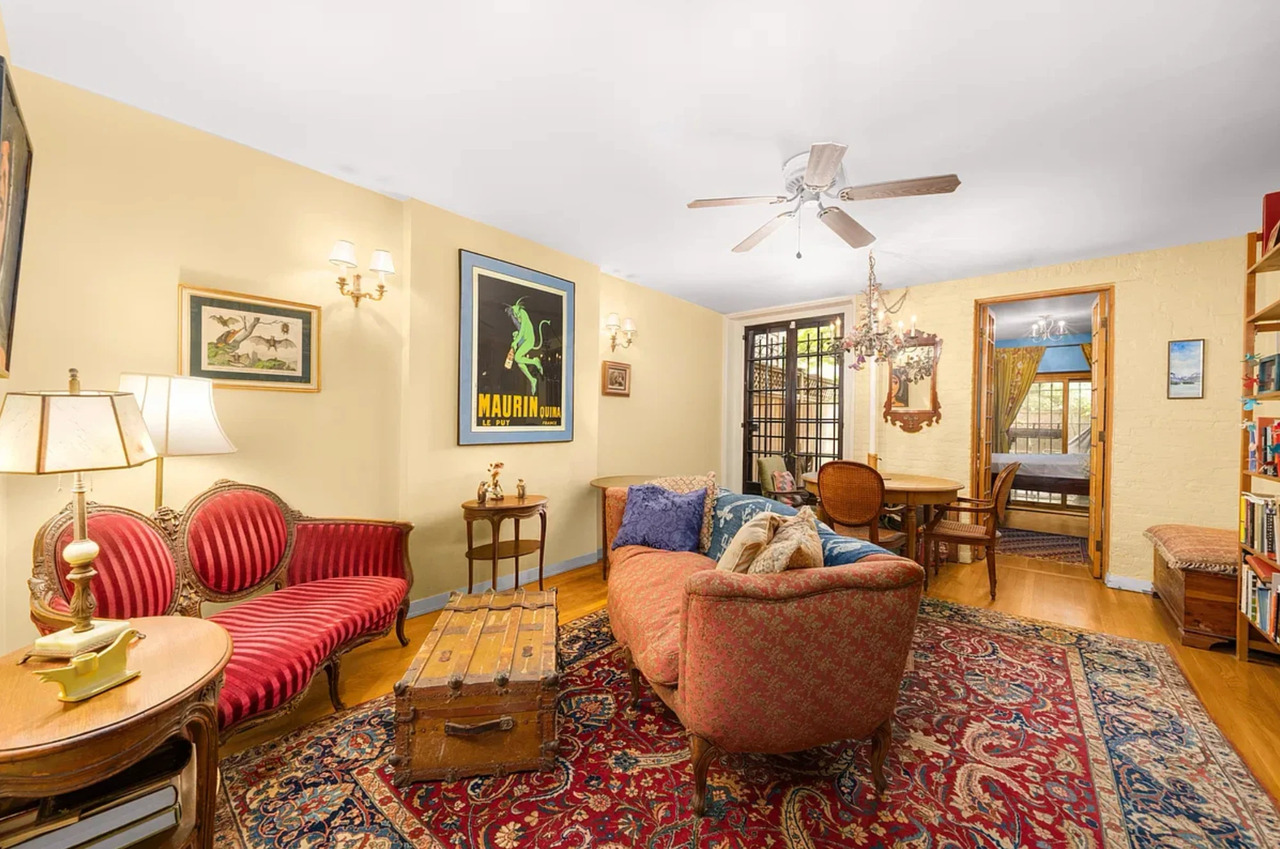
\includegraphics[width=\linewidth]{uws_interior.jpg}
      \credit{Listing photo: StreetEasy}
    \end{column}
  \end{columns}
  \source{Source: \href{https://streeteasy.com/building/306-west-90-street-new_york/1}{listing for 306 West 90th Street \#1} (StreetEasy / Nest Seekers, Nov.\ 2026). Median Manhattan sale, Q3 2026: \$1,275,000 (UrbanDigs).}
\end{frame}

\photoslide{Upper West Side}{uws_street.jpg}{Brownstones, West 69th Street. Photo: Tony Hisgett, CC BY 2.0}
  {\item Riverside Park: around the corner
   \item Subway: 5 minutes' walk
   \item Museums, theaters, restaurants
   \item \alert{No car} needed}
  {}

\begin{thinkframe}
  {\color{oldred}\textbf{Think}}\\[0.8em]
  Same price. Which one would \alert{you} buy?\\[0.3em] Why?
\end{thinkframe}

% =====================================================================
\section{Why New York?}

\begin{frame}{Ask a New Yorker}
  \centering
  \relax{\color{muted} Why do people live in New York?\par}
  \vspace{0.3em}
  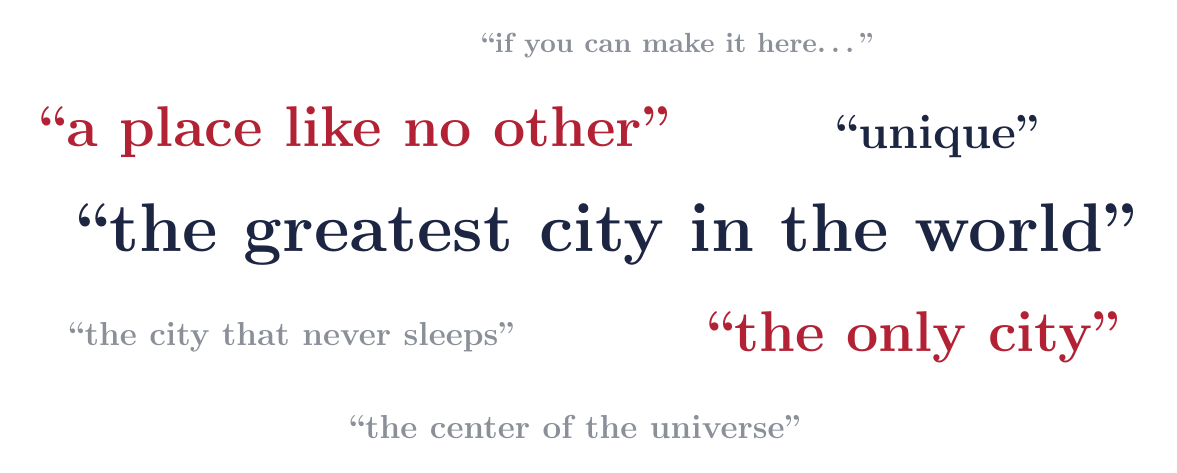
\begin{tikzpicture}[every node/.style={font=\bfseries, inner sep=2pt}]
    \node[font=\Huge\bfseries, text=navy] at (0,0) {``the greatest city in the world''};
    \node[font=\huge\bfseries, text=oldred] at (-3.2,1.3) {``a place like no other''};
    \node[font=\huge\bfseries, text=oldred] at (3.9,-1.3) {``the only city''};
    \node[font=\LARGE\bfseries, text=navy] at (4.2,1.25) {``unique''};
    \node[font=\large\bfseries, text=muted] at (-4.0,-1.3) {``the city that never sleeps''};
    \node[font=\large\bfseries, text=muted] at (-0.4,-2.45) {``the center of the universe''};
    \node[font=\normalsize\bfseries, text=muted] at (0.9,2.4) {``if you can make it here\ldots''};
  \end{tikzpicture}
\end{frame}

\begin{frame}{What they really mean}
  \vspace{1.2cm}
  \begin{columns}[T]
    \begin{column}{0.45\textwidth}\centering
      {\fontsize{36}{40}\selectfont\bfseries\color{navy} Density}
    \end{column}
    \begin{column}{0.45\textwidth}\centering
      {\fontsize{36}{40}\selectfont\bfseries\color{oldred} Possibility}
    \end{column}
  \end{columns}
\end{frame}

% =====================================================================
\section{Density}

\begin{frame}{Density in numbers}
  \vspace{0.8cm}
  \begin{columns}[T]
    \begin{column}{0.3\textwidth}\bignum{navy}{8.6\,M}{people}\end{column}
    \begin{column}{0.3\textwidth}\bignum{navy}{778}{km\textsuperscript{2} (300 square miles)}\end{column}
    \begin{column}{0.3\textwidth}\bignum{oldred}{11,300}{people per km\textsuperscript{2}}\end{column}
  \end{columns}
  \source{Source: US Census Bureau (2025 estimate; land area), via Wikipedia.}
\end{frame}

\begin{frame}{New York vs.\ Austria}
  \centering
  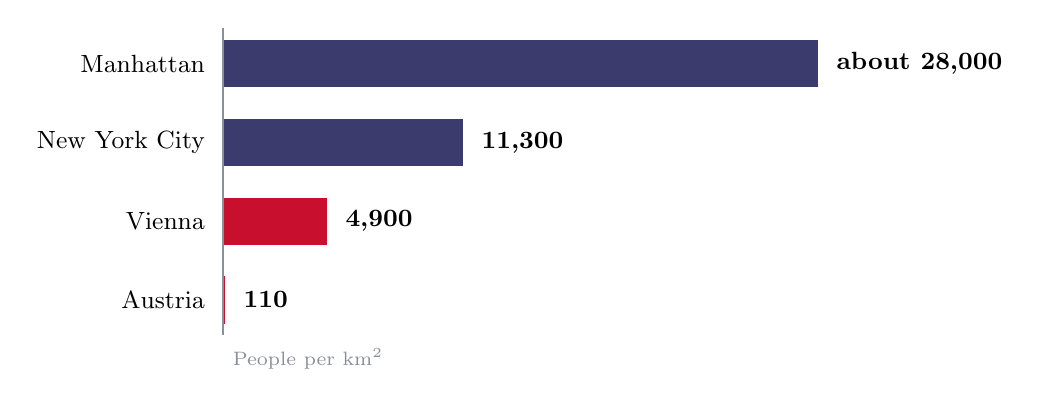
\begin{tikzpicture}[x=0.27cm, y=-1.0cm]   % 1 unit = 1,000 people per km2
    \foreach \y/\lab/\val/\txt/\col in {
        0/Manhattan/28/{about 28,000}/oldblue,
        1/New York City/11.3/{11,300}/oldblue,
        2/Vienna/4.9/{4,900}/austria,
        3/Austria/0.11/{110}/austria} {
      \fill[\col] (0,\y) rectangle (\val,\y+0.6);
      \node[anchor=east, font=\small] at (-0.4,\y+0.3) {\lab};
      \node[anchor=west, font=\small\bfseries] at (\val+0.4,\y+0.3) {\txt};
    }
    \draw[muted] (0,-0.15) -- (0,3.75);
    \node[font=\scriptsize, text=muted, anchor=west] at (0,4.05) {People per km\textsuperscript{2}};
  \end{tikzpicture}

  \vspace{0.5em}
  All of Austria's people, in a space \alert{twice the size of Vienna}.
  \source{Sources: US Census Bureau; Statistik Austria (1 Jan.\ 2026: Austria 9,215,956, Vienna 2,040,914).}
\end{frame}

\photoslide{Everything is close}{subway2.jpg}{Photo: Martin David, CC0}
  {\item \alert{472} subway stations
   \item Open 24 hours a day
   \item \alert{56\%} of households: no car
   \item Groceries, school, work: walking distance}
  {Sources: MTA; US Census Bureau (American Community Survey), via Vital City.}

% =====================================================================
\section{Possibility}

\begin{frame}{Something for everyone}
  \vspace{0.4cm}
  \begin{columns}[T]
    \begin{column}{0.4\textwidth}\bignum{oldred}{36\%}{of New Yorkers born abroad}\end{column}
    \begin{column}{0.4\textwidth}\bignum{navy}{800}{languages spoken}\end{column}
  \end{columns}
  \vspace{1.2em}
  \begin{center}
  \begin{minipage}{0.5\textwidth}
    \begin{itemize}\setlength{\itemsep}{0.5em}
      \item Food from every country
      \item Every job, every hobby, every scene
    \end{itemize}
  \end{minipage}
  \end{center}
  \source{Sources: American Community Survey 2024 (via Data USA); Endangered Language Alliance (via Wikipedia).}
\end{frame}

\begin{frame}{Game: Can you find it in New York?}
  \relax{\color{muted} Teams: write \textbf{yes} or \textbf{no} for each.\par}
  \vspace{0.6em}
  \begin{columns}[T]
    \begin{column}{0.5\textwidth}
      \begin{enumerate}\setlength{\itemsep}{0.7em}
        \item A beach where you can surf
        \item A working farm
        \item A Viennese caf\'e with Sachertorte
      \end{enumerate}
    \end{column}
    \begin{column}{0.45\textwidth}
      \begin{enumerate}\setlength{\itemsep}{0.7em}\setcounter{enumi}{3}
        \item A castle
        \item Wild coyotes
        \item A ski slope
      \end{enumerate}
    \end{column}
  \end{columns}
\end{frame}

\begin{frame}{Answers}
  \begin{columns}[c]
    \begin{column}{0.6\textwidth}
      \begin{enumerate}\setlength{\itemsep}{0.55em}
        \item Surf beach? \uncover<2->{\alert{\textbf{Yes:}} Rockaway, Queens}
        \item Farm? \uncover<3->{\alert{\textbf{Yes:}} Queens County Farm (1697)}
        \item Viennese caf\'e? \uncover<4->{\alert{\textbf{Yes:}} Caf\'e Sabarsky}
        \item Castle? \uncover<5->{\alert{\textbf{Yes:}} Belvedere Castle}
        \item Coyotes? \uncover<6->{\alert{\textbf{Yes:}} even in Central Park}
        \item Ski slope? \uncover<7->{\textbf{No:} leave the city}
      \end{enumerate}
    \end{column}
    \begin{column}{0.36\textwidth}
      \centering
      \only<2>{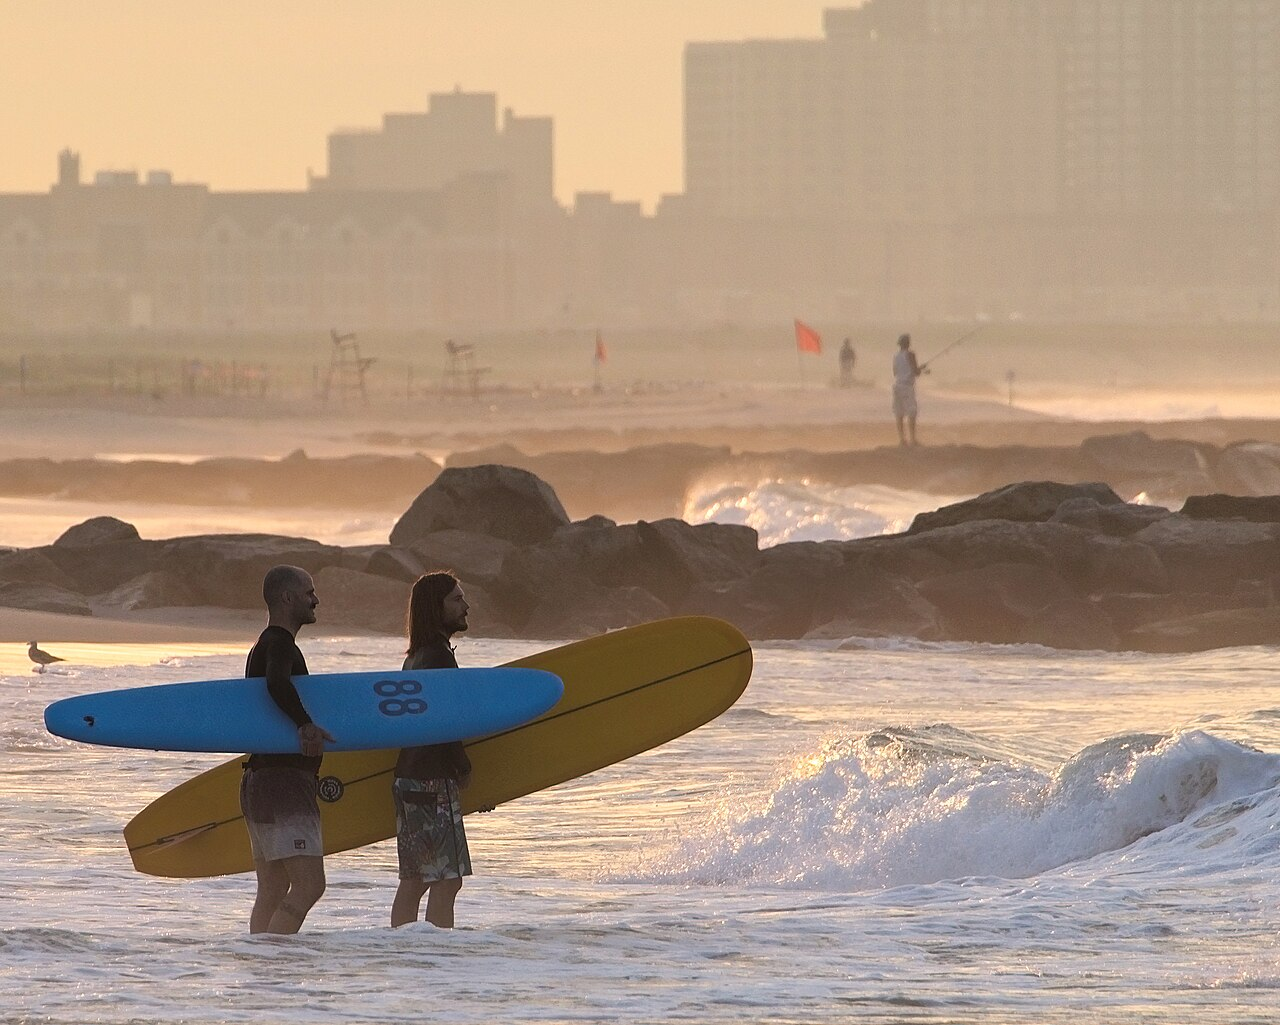
\includegraphics[width=\linewidth]{rockaway.jpg}\credit{Rockaway Beach. Photo: joiseyshowaa, CC BY-SA 2.0}}%
      \only<3>{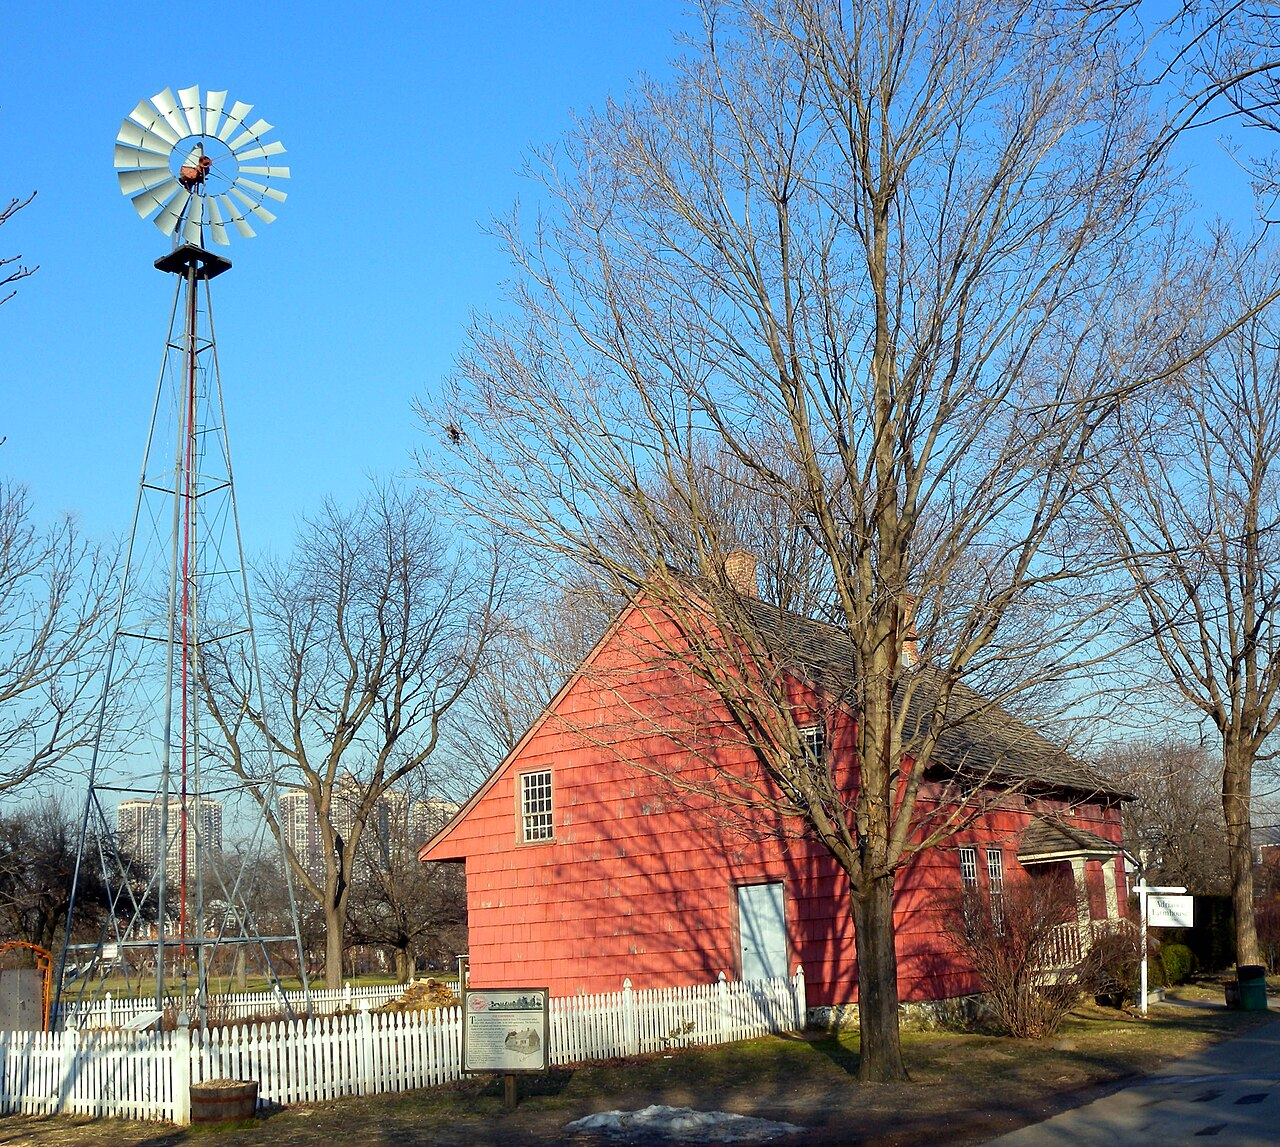
\includegraphics[height=5cm]{qfarm.jpg}\credit{Queens County Farm. Photo: Jim Henderson, public domain}}%
      \only<5>{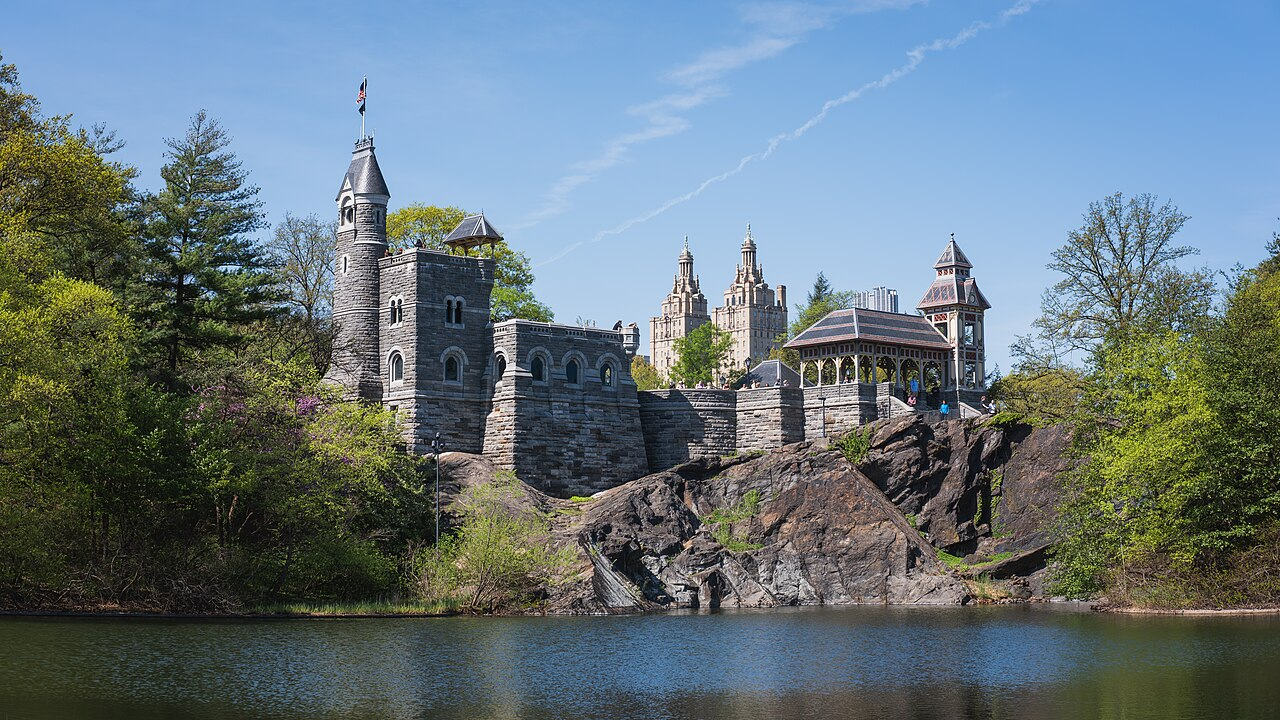
\includegraphics[width=\linewidth]{belvedere.jpg}\credit{Belvedere Castle. Photo: Christian David, CC BY-SA 4.0}}%
      \only<6>{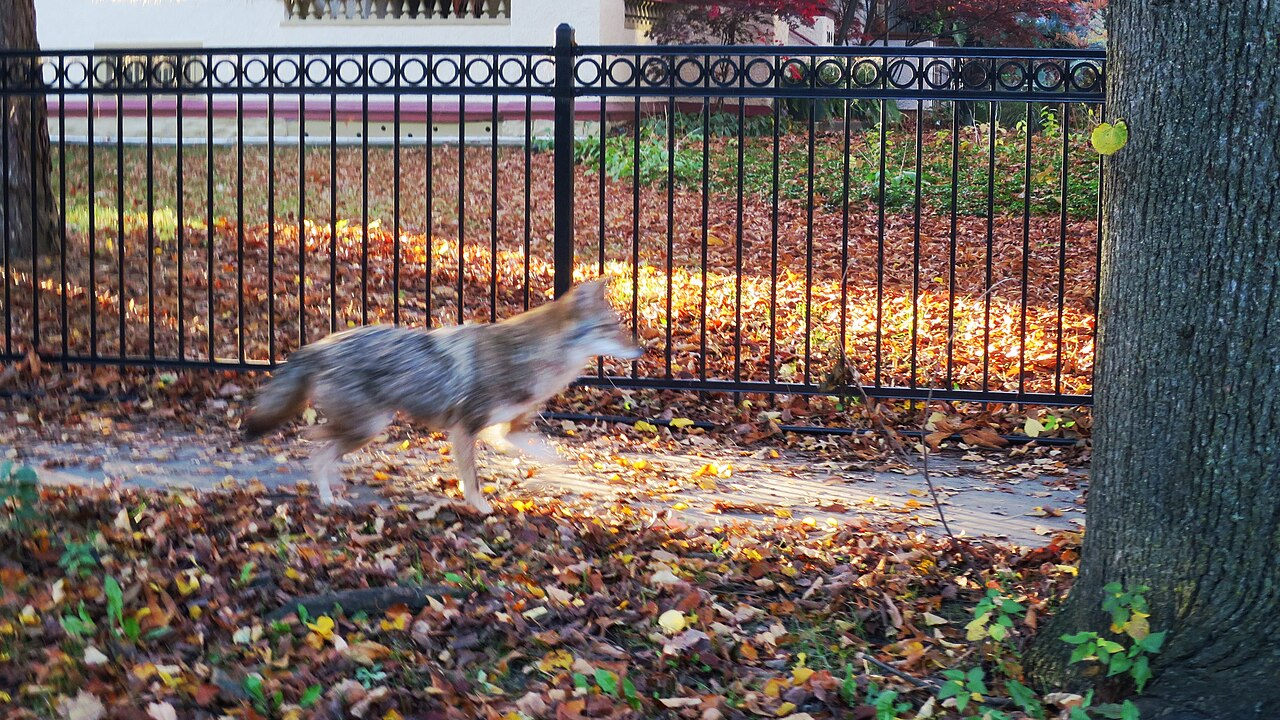
\includegraphics[width=\linewidth]{coyote.jpg}\credit{A coyote. Photo: Brian Crawford, CC BY-SA 2.0}}%
    \end{column}
  \end{columns}
\end{frame}

% =====================================================================
\section{Five Boroughs, One Budget}

\begin{frame}{Remember our apartment?}
  \begin{columns}[c]
    \begin{column}{0.5\textwidth}
      \begin{itemize}\setlength{\itemsep}{0.9em}
        \item I said: this is New York
        \item Only \alert{one} option
        \item Same \alert{\$1.2 million}, five boroughs
      \end{itemize}
    \end{column}
    \begin{column}{0.42\textwidth}
      \centering
      \begin{tikzpicture}
        \node[inner sep=0pt, anchor=south west] (m) at (0,0) {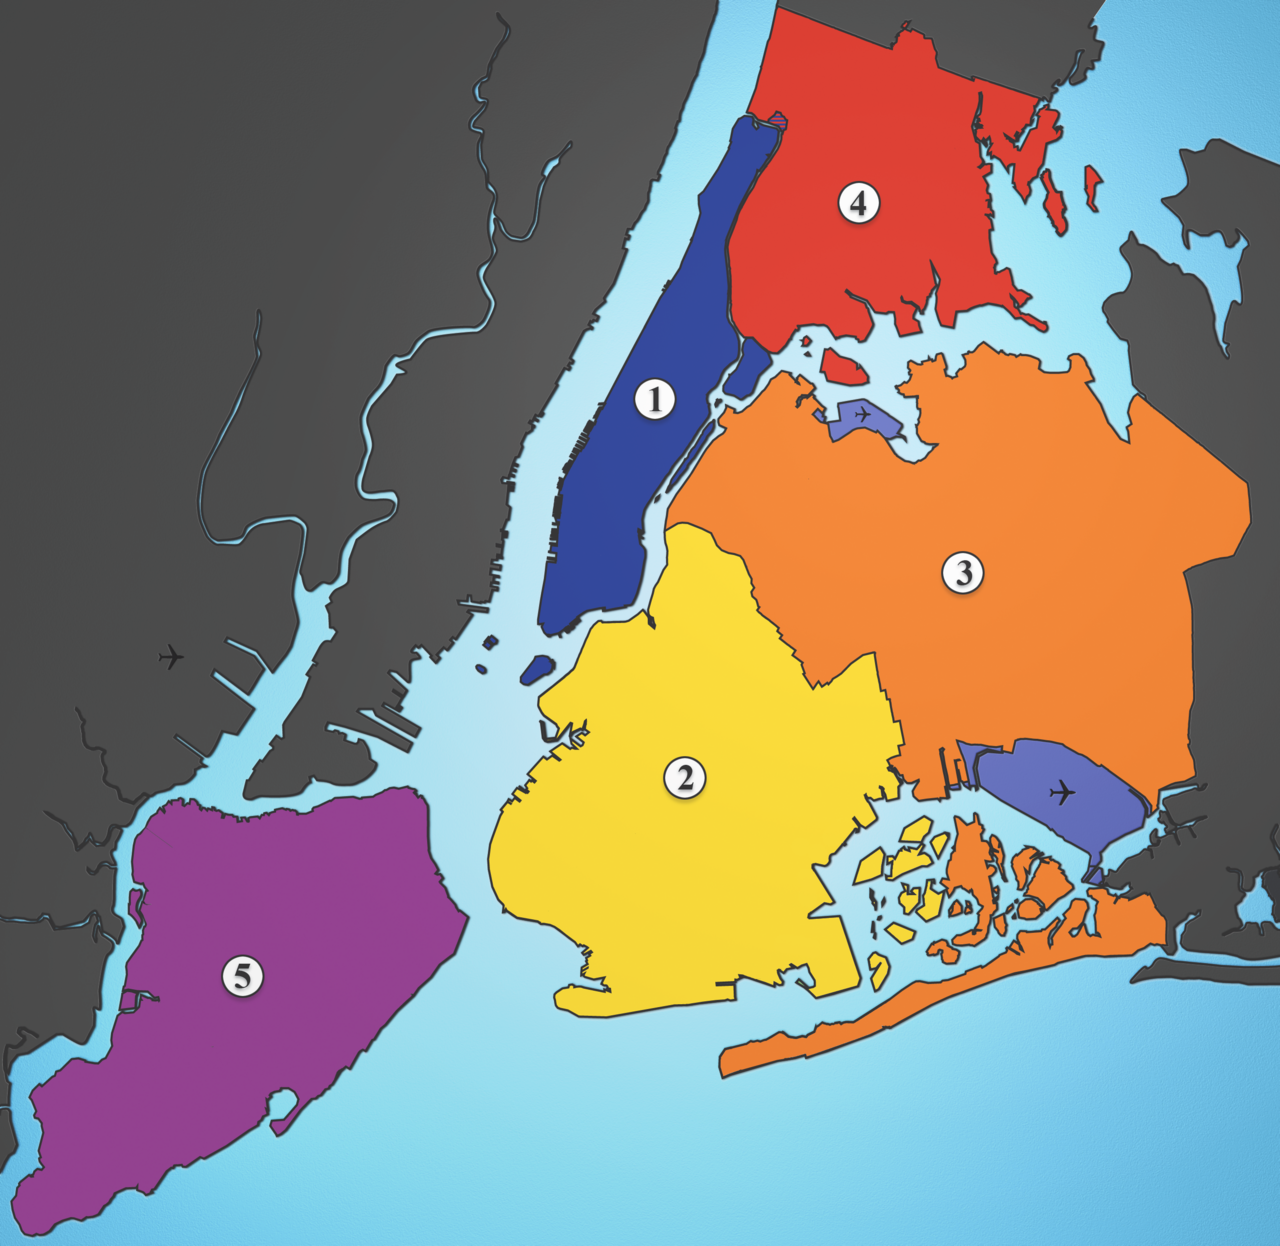
\includegraphics[width=5.2cm]{boroughs.png}};
        \begin{scope}[x={(m.south east)}, y={(m.north west)}, every node/.style={font=\scriptsize\bfseries, fill=white, fill opacity=0.85, text opacity=1, inner sep=1.5pt, rounded corners=1pt}]
          \node at (0.36,0.70) {Manhattan};
          \node at (0.47,0.30) {Brooklyn};
          \node at (0.67,0.50) {Queens};
          \node at (0.63,0.89) {Bronx};
          \node at (0.17,0.12) {Staten Island};
        \end{scope}
      \end{tikzpicture}
      \credit{Map: Wikimedia Commons, CC BY-SA 2.5}
    \end{column}
  \end{columns}
\end{frame}

\photoslide{Manhattan}{uws_listing.jpg}{306 West 90th Street. Listing photo: StreetEasy}
  {\item A 2-bedroom apartment
   \item About 86 m\textsuperscript{2}
   \item A tiny garden, if you're lucky}
  {Source: UrbanDigs / Keller Williams NYC, Q3 2026 (median sale \$1,275,000).}

\photoslide{Brooklyn}{parkslope.jpg}{Park Slope. Photo: David Berkowitz, CC BY 2.0}
  {\item \alert{One floor} of a brownstone
   \item Park Slope: trees, families, caf\'es
   \item Prospect Park nearby}
  {Source: Milton Coste / REBNY, Q3 2026 (Park Slope median, all homes: \$1,782,500).}

\photoslide{Queens}{queens.jpg}{Attached houses, Ridgewood. Photo: Jim Henderson, public domain}
  {\item A whole \alert{attached} house
   \item 3 bedrooms, small backyard
   \item Neighbors on both sides}
  {Source: Milton Coste / REBNY, Q3 2026 (Queens house median: \$1,150,000).}

\photoslide{Staten Island}{statenisland.jpg}{Westerleigh. Photo: Andre Carrotflower, CC BY-SA 4.0}
  {\item A \alert{detached} house
   \item Driveway, garage, garden
   \item Feels like the suburbs
   \item Ferry to Manhattan: \alert{free}}
  {Source: DeFalco Realty, May 2026 (Staten Island single-family median: about \$795,000).}

\photoslide{The Bronx}{bronx.jpg}{Throgs Neck. Photo: Tdorante10, CC BY-SA 4.0}
  {\item A \alert{two-family} house
   \item Live upstairs, rent out downstairs
   \item Yankee Stadium, the Bronx Zoo}
  {Source: NYC Department of Finance, 2025 sales (Bronx two-family median: \$815,000).}

\begin{frame}{Vote: where would you live?}
  \centering
  \vspace{0.3cm}
  \bthumb{uws_listing.jpg}{Manhattan}\hfill
  \bthumb{parkslope.jpg}{Brooklyn}\hfill
  \bthumb{queens.jpg}{Queens}\hfill
  \bthumb{statenisland.jpg}{Staten Island}\hfill
  \bthumb{bronx.jpg}{The Bronx}

  \vspace{1.5em}
  {\Large Stand next to your borough. \alert{Why?}}
\end{frame}

% =====================================================================
\section{Neighborhoods of Manhattan}

\begin{frame}{One borough, many worlds}
  \centering
  \begin{tikzpicture}
    \node[inner sep=0pt, anchor=south west] (m) at (0,0) {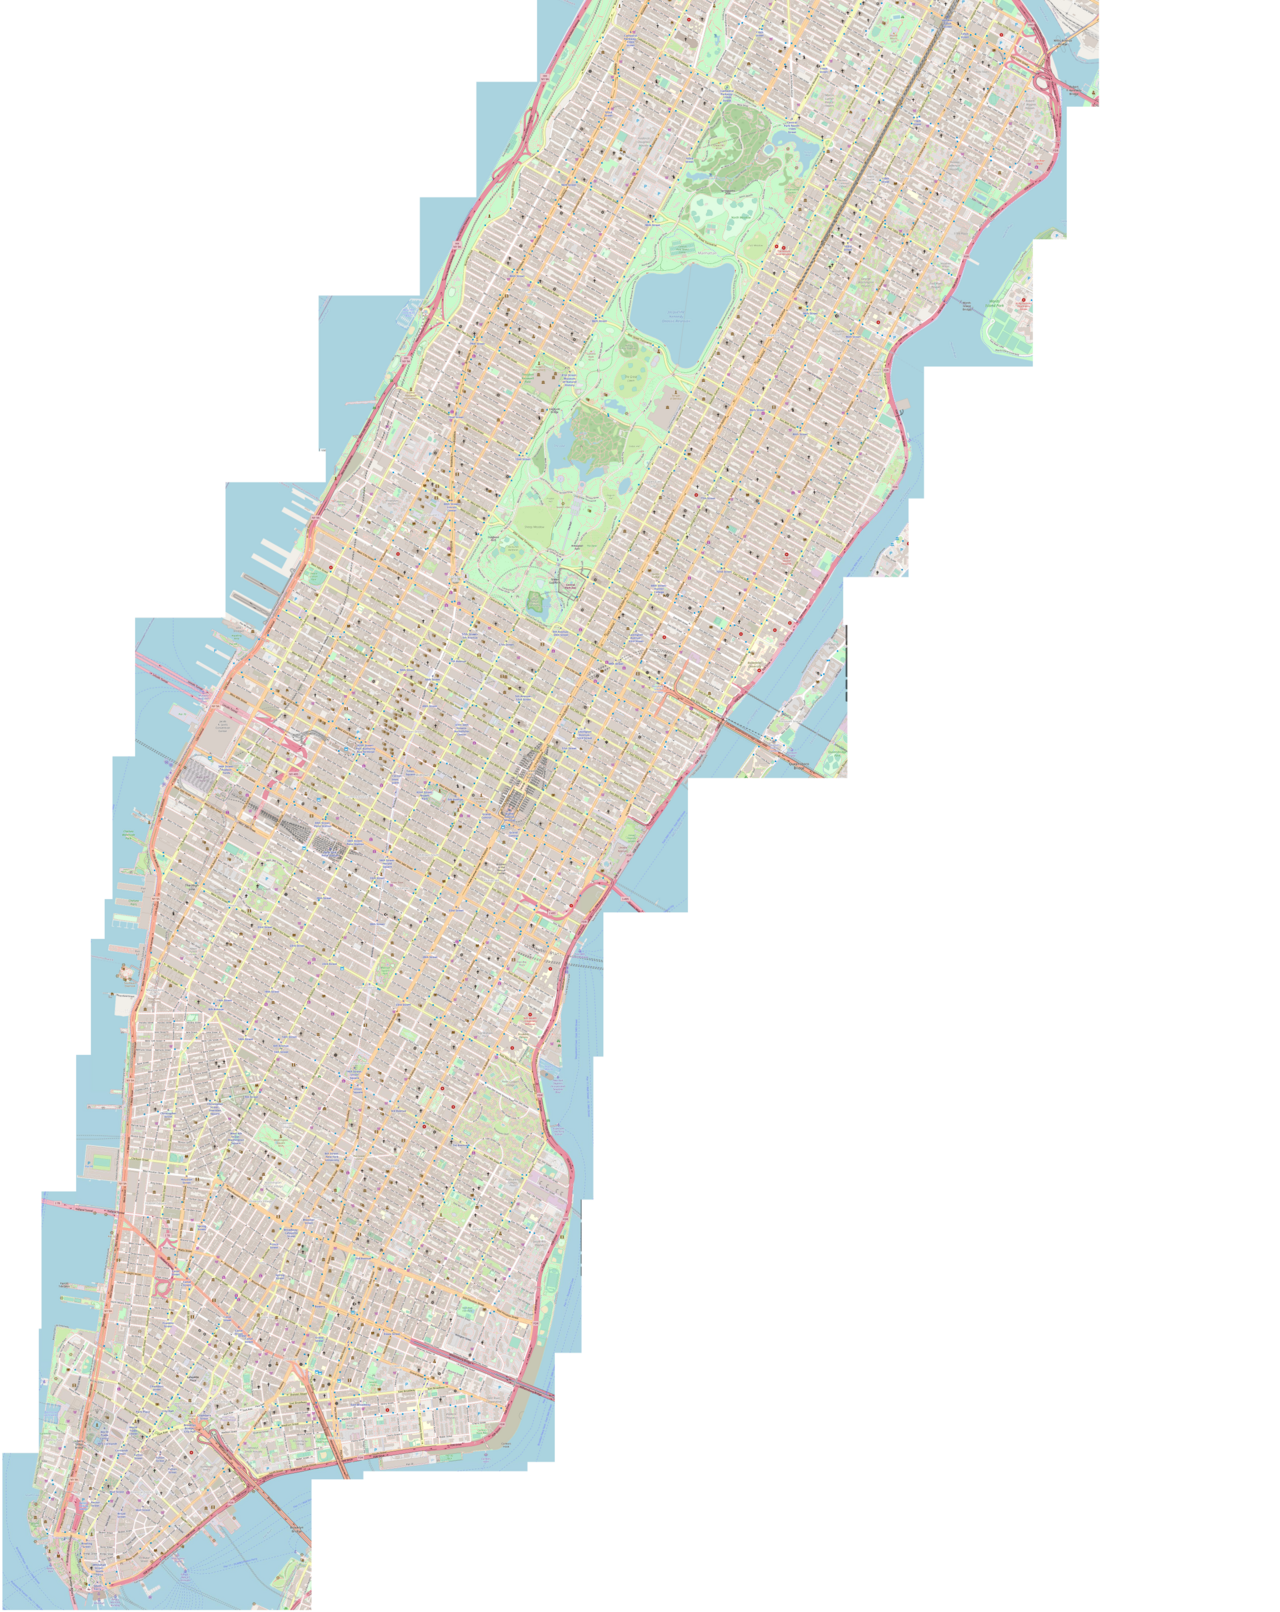
\includegraphics[height=5.9cm]{manhattan_map.png}};
    \begin{scope}[x={(m.south east)}, y={(m.north west)}]
      \hood{510}{320}{-0.45}{0.82}{east}{Upper West Side}
      \hood{420}{745}{-0.45}{0.55}{east}{Midtown}
      \hood{210}{900}{-0.45}{0.42}{east}{Chelsea}
      \hood{155}{1090}{-0.45}{0.29}{east}{West Village}
      \hood{245}{1235}{-0.45}{0.17}{east}{SoHo}
      \hood{190}{1500}{-0.45}{0.05}{east}{Wall Street}
      \hood{820}{345}{1.25}{0.80}{west}{Upper East Side}
      \hood{480}{1145}{1.25}{0.32}{west}{\shortstack[l]{East Village /\\Lower East Side}}
      \hood{365}{1310}{1.25}{0.17}{west}{Chinatown}
    \end{scope}
  \end{tikzpicture}
  \credit{Map: \copyright\ OpenStreetMap contributors}
\end{frame}

\photoslide{Upper West Side}{amnh.jpg}{American Museum of Natural History. Photo: Ferfive, CC BY 4.0}
  {\item Between \alert{two parks}
   \item Pre-war apartments, brownstones
   \item Families, dogs, strollers
   \item Natural History Museum}
  {}

\photoslide{Upper East Side}{met.jpg}{The Metropolitan Museum of Art. Photo: Hugo Schneider, CC BY-SA 2.0}
  {\item ``\alert{Old money}'' New York
   \item Fifth Avenue, Park Avenue
   \item Museum Mile: the Met
   \item \emph{Gossip Girl}}
  {}

\photoslide{Midtown}{timessq.jpg}{Times Square. Photo: Nkon21, CC BY-SA 4.0}
  {\item Times Square, Broadway
   \item Empire State Building
   \item Grand Central Terminal
   \item Offices, tourists, \alert{crowds}}
  {}

\photoslide{Chelsea}{highline.jpg}{The High Line. Photo: Rob Young, CC BY 2.0}
  {\item \alert{Art galleries} everywhere
   \item The High Line: park on old train tracks
   \item Chelsea Market
   \item Center of gay New York}
  {}

\photoslide{West Village}{westvillage.jpg}{West 4th Street. Photo: Kidfly182, CC BY-SA 4.0}
  {\item Crooked streets, \alert{no grid}
   \item Small townhouses, tiny restaurants
   \item Stonewall Inn: gay rights, 1969
   \item The \emph{Friends} building}
  {}

\photoslide{East Village / Lower East Side}{tenement.jpg}{97 Orchard Street, now the Tenement Museum. Photo: Sdkb, CC BY-SA 4.0}
  {\item Once: \alert{immigrant} tenements
   \item Then: punk, artists, cheap rent
   \item Now: bars and nightlife
   \item Katz's Deli, since 1888}
  {}

\photoslide{SoHo}{soho.jpg}{Cast-iron buildings. Photo: 50greenestreet, CC BY-SA 4.0}
  {\item ``\alert{So}uth of \alert{Ho}uston'' Street
   \item Say it: \textbf{HOW-ston}
   \item Cast-iron buildings
   \item Artists' lofts, now shops}
  {}

\photoslide{Chinatown}{chinatown.jpg}{Mott Street. Photo: Frank Schulenburg, CC BY-SA 4.0}
  {\item One of the biggest \alert{outside Asia}
   \item Dumplings, markets, temples
   \item Canal Street
   \item Little Italy next door}
  {}

\photoslide{Wall Street}{wtc.jpg}{One World Trade Center. Photo: Christian David, CC BY-SA 4.0}
  {\item Named after a \alert{real wall} (1650s)
   \item New York Stock Exchange
   \item 9/11 Memorial
   \item One World Trade Center: 541 m}
  {}

% =====================================================================
\section{Your Turn}

\begin{frame}{Your \$1.2 million}
  \centering
  {\Large You have \alert{\$1.2 million}. Where do you buy?}\\[1.2em]
  \begin{minipage}{0.62\textwidth}
    \begin{itemize}\setlength{\itemsep}{0.8em}
      \item The \href{https://www.nestseekers.com/5535527/beautifully-renovated-farmhouse-on-22-private-acres-with-a-heated}{Hudson farmhouse}?
      \item The \href{https://streeteasy.com/building/306-west-90-street-new_york/1}{Upper West Side apartment}?
      \item Or which borough and neighborhood?
      \item One reason: \alert{density} or \alert{possibility}?
    \end{itemize}
  \end{minipage}
\end{frame}

\end{document}
